\chapter{User Guide}
\section{Instructions}
\begin{enumerate}
    \item When the application is started, you will be displayed with the homepage (Figure \ref{fig:sc1}).
    \item Press the ``Sign in with GitHub" button to login to the application.
    \item An external page from GitHub will appear (Figure \ref{fig:sc7}). Press the green ``Authorize" button.
    \item You will then be redirected back to the application. A list of all repositories you are a contributor to (both private and public) will be listed (Figure \ref{fig:sc2}).
    \item Click on the name of the repository you want analysed. 
    \item Depending on the size of the repository, there may be a large wait until the next page is reached due to the calculations taking place. Wait until the next page is displayed.
    \item The displayed page will show the visualisations of contributions with a pie chart showing percentage of contributions and a bar chart showing the persistence score for each user, as seen in Figure \ref{fig:sc3}.
    \item There is a sidebar with two clickable options: Team View and File View. Click on the ``Team View" option.
    \item The page will be reloaded and instead of showing all users' contributions, it will show your contributions in relation to the rest of the team (Figure \ref{fig:sc4}).
    \item Click on the ``File View" button. This will show a list of all the files in the selected repository (Figure \ref{fig:sc5}).
    \item Click on any file that you want analysing. This will load a new visualisation that highlights each user's contribution per file per character as seen in Figure \ref{fig:sc6}.
\end{enumerate}

\begin{figure}
    \centering
    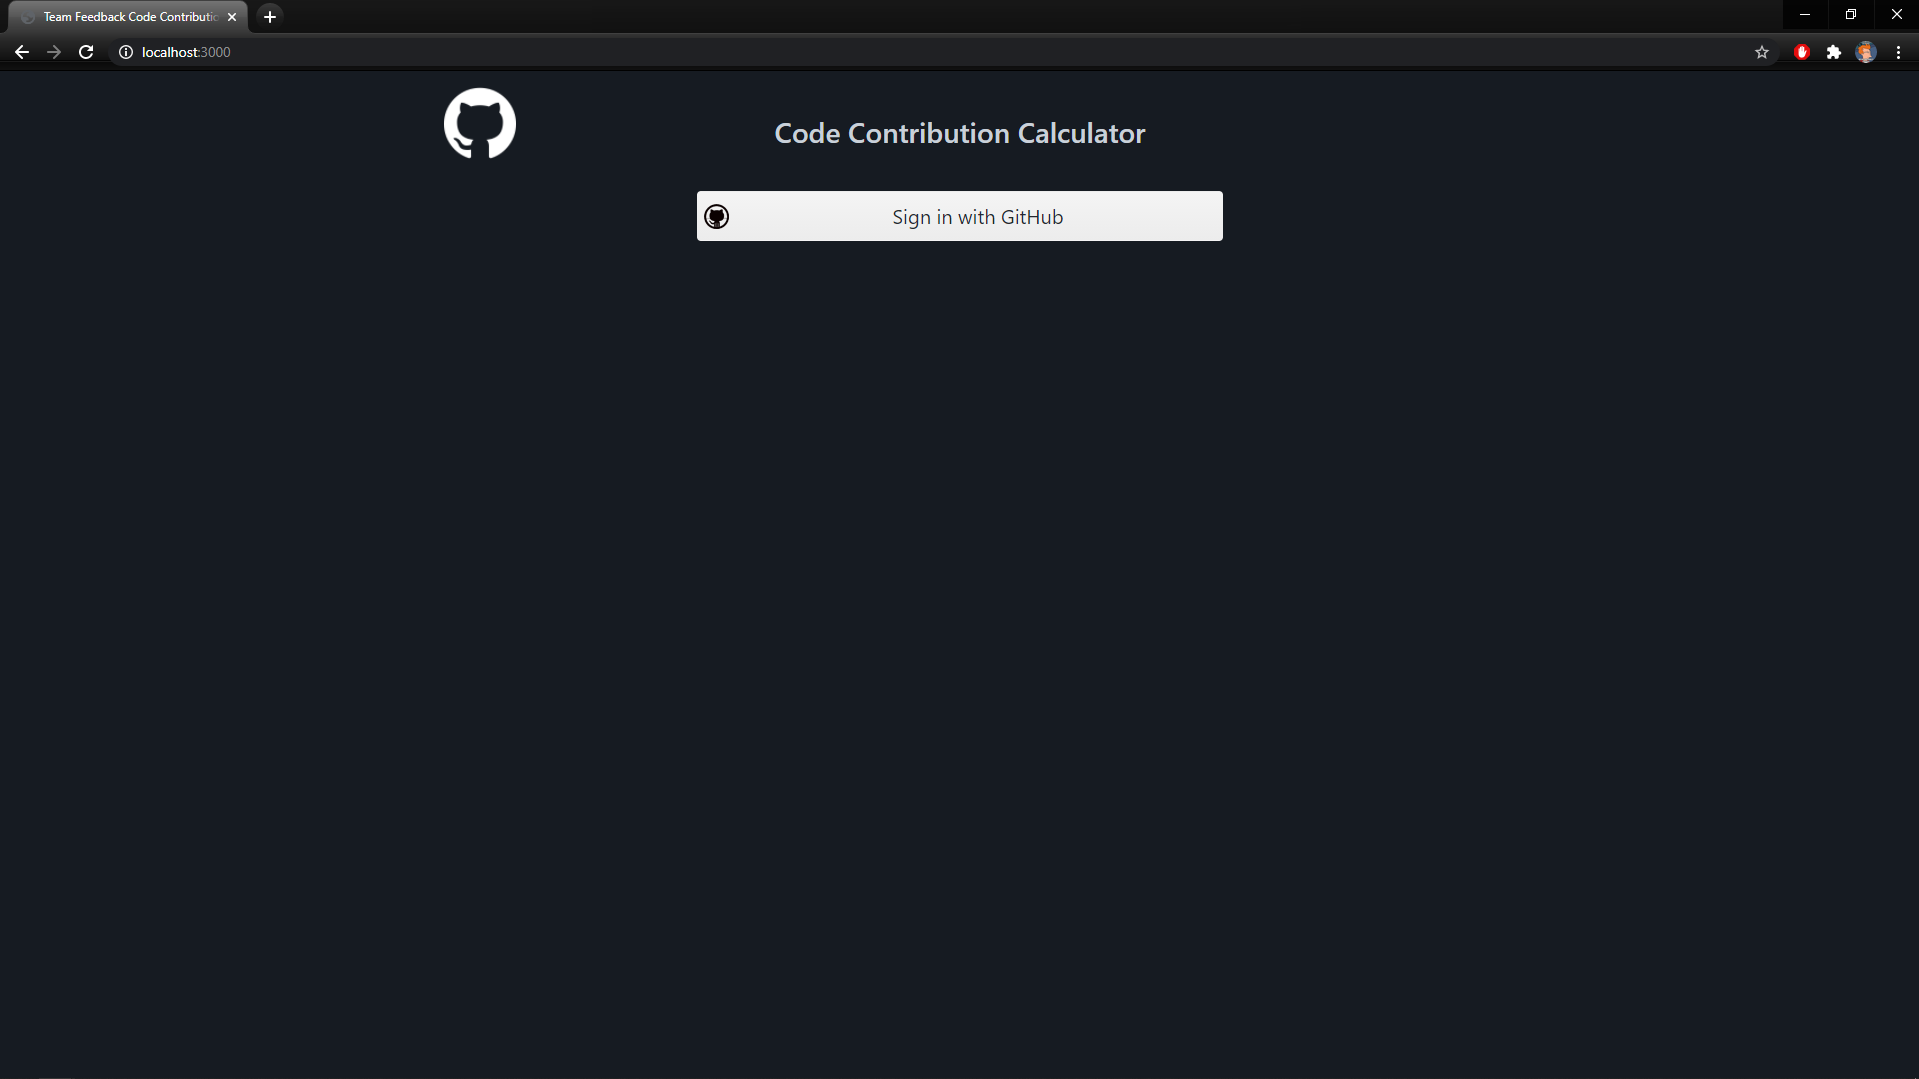
\includegraphics[scale=0.3]{Appendices/Screenshot_92.png}
    \caption{Homepage}
    \label{fig:sc1}
\end{figure}
\begin{figure}
    \centering
    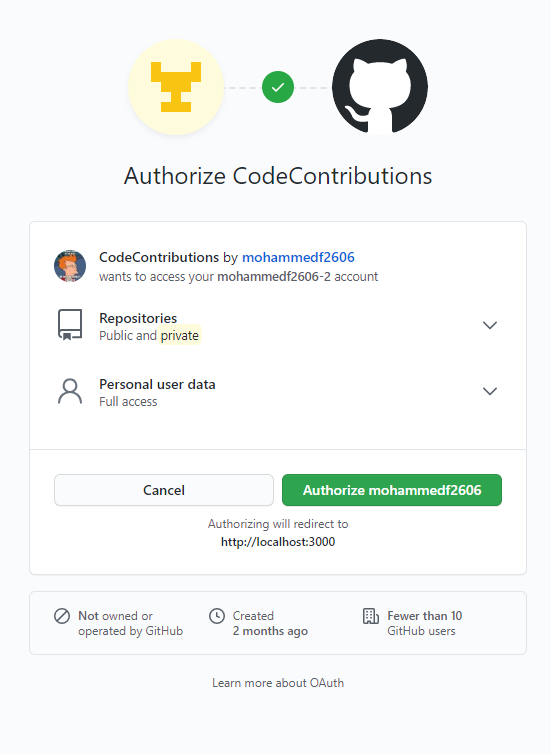
\includegraphics[scale=0.6]{Appendices/Screenshot_98.png}
    \caption{GitHub authorisation page}
    \label{fig:sc7}
\end{figure}
\begin{figure}
    \centering
    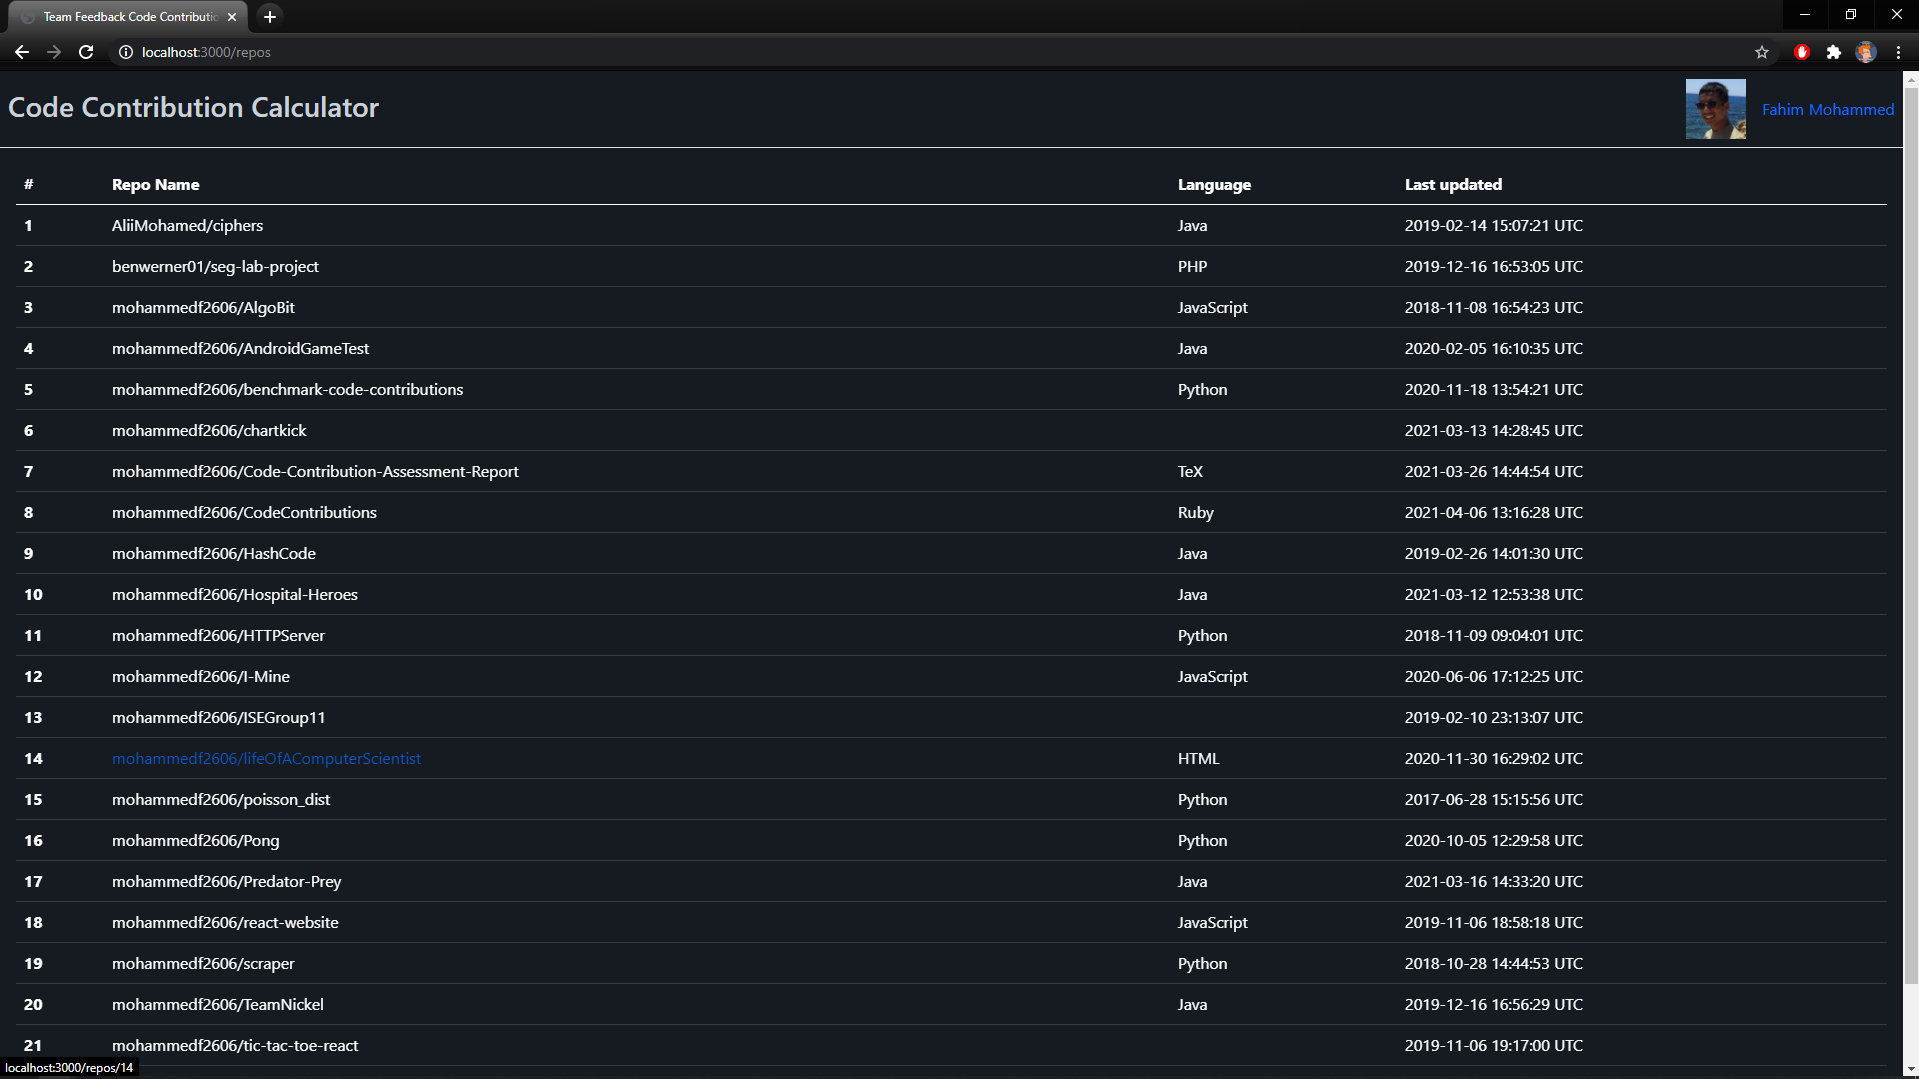
\includegraphics[scale=0.3]{Appendices/Screenshot_93.png}
    \caption{Repository list}
    \label{fig:sc2}
\end{figure}
\begin{figure}
    \centering
    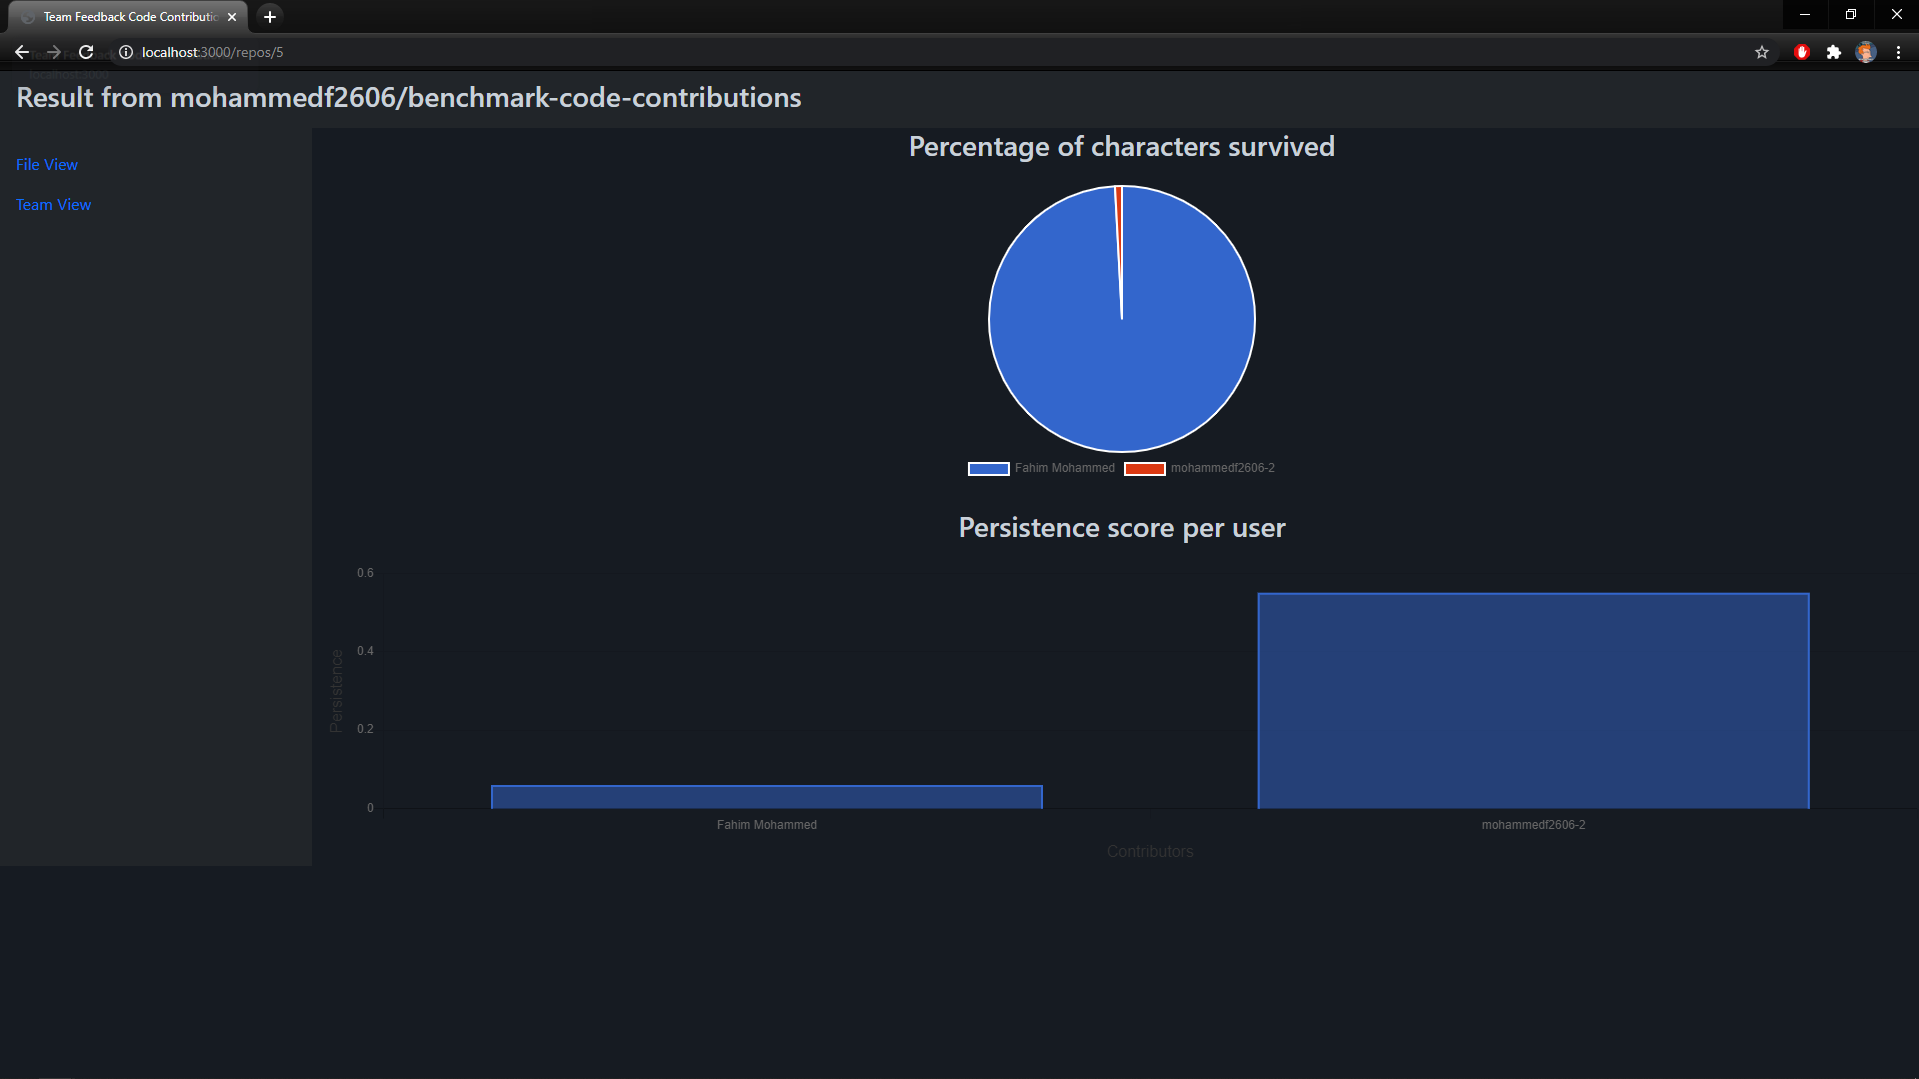
\includegraphics[scale=0.3]{Appendices/Screenshot_94.png}
    \caption{Repository results}
    \label{fig:sc3}
\end{figure}
\begin{figure}
    \centering
    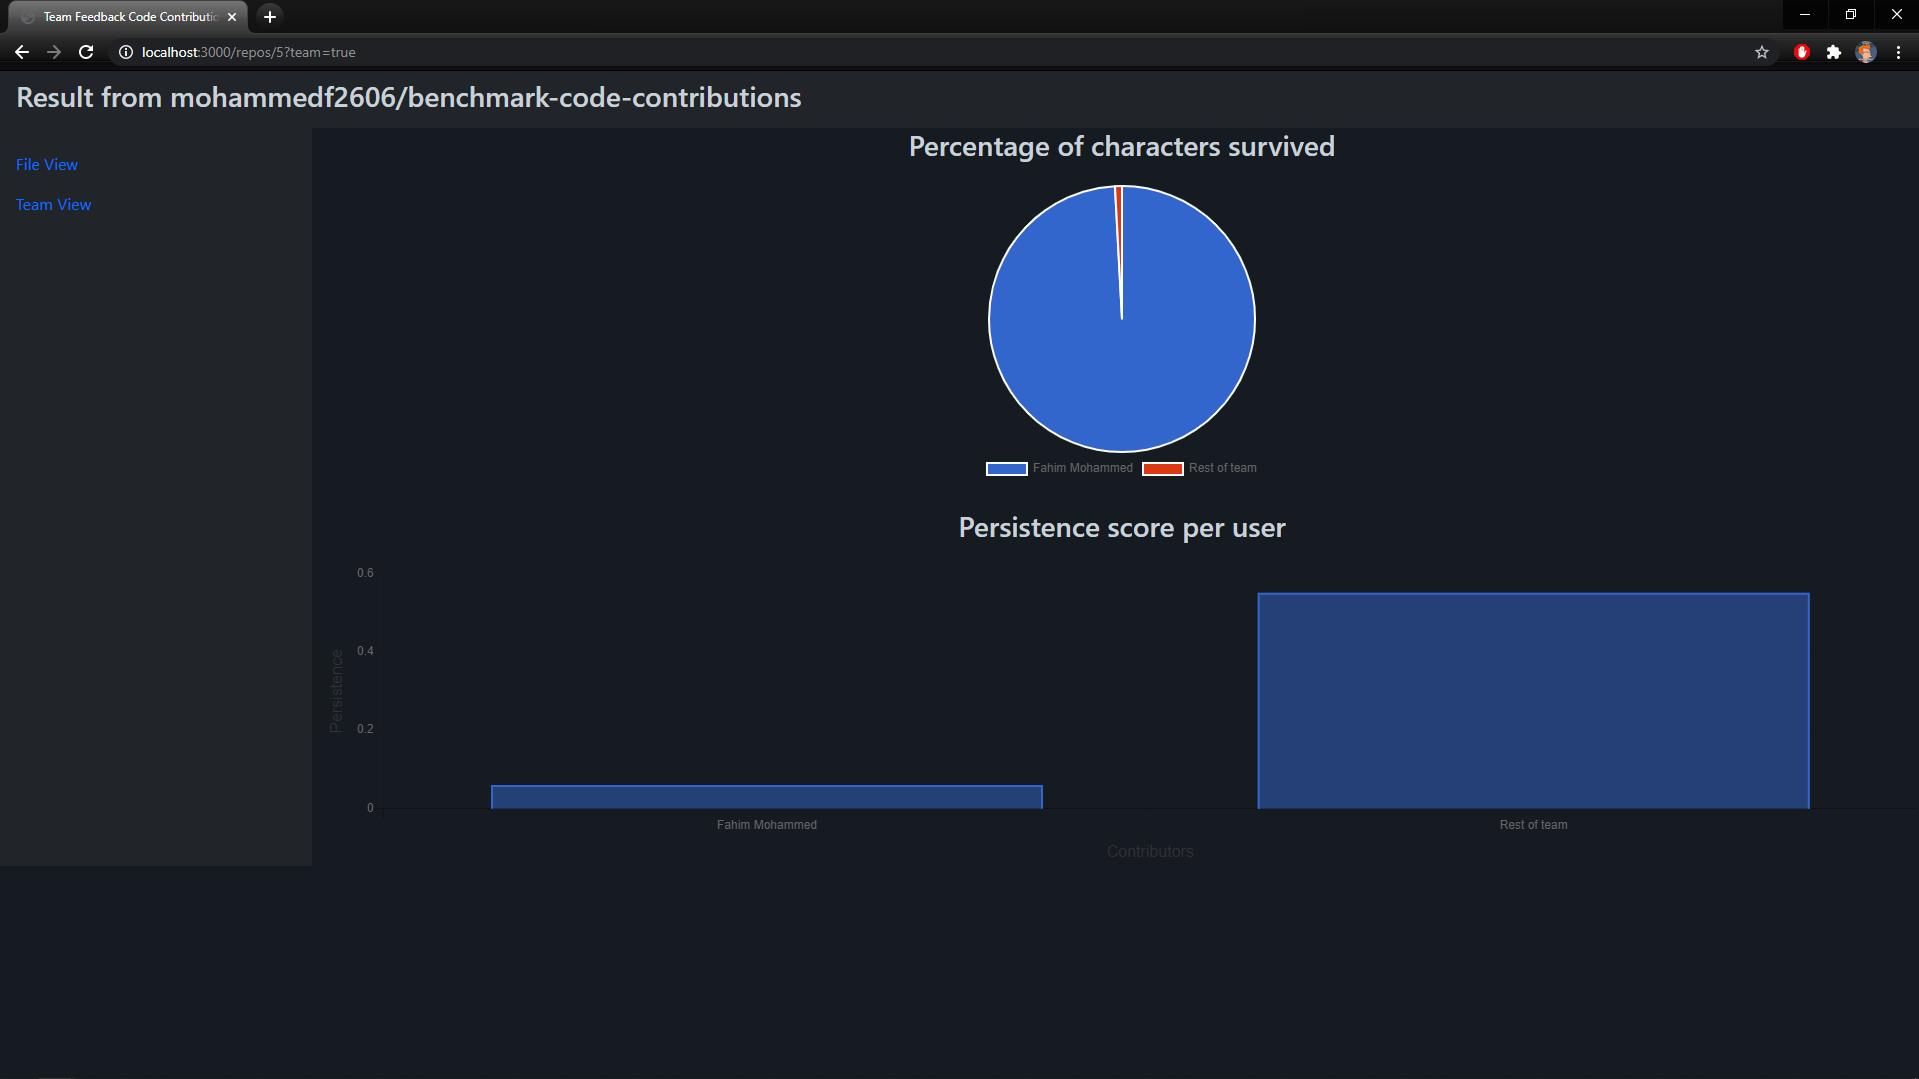
\includegraphics[scale=0.3]{Appendices/Screenshot_95.png}
    \caption{Repository results with team view on}
    \label{fig:sc4}
\end{figure}
\begin{figure}
    \centering
    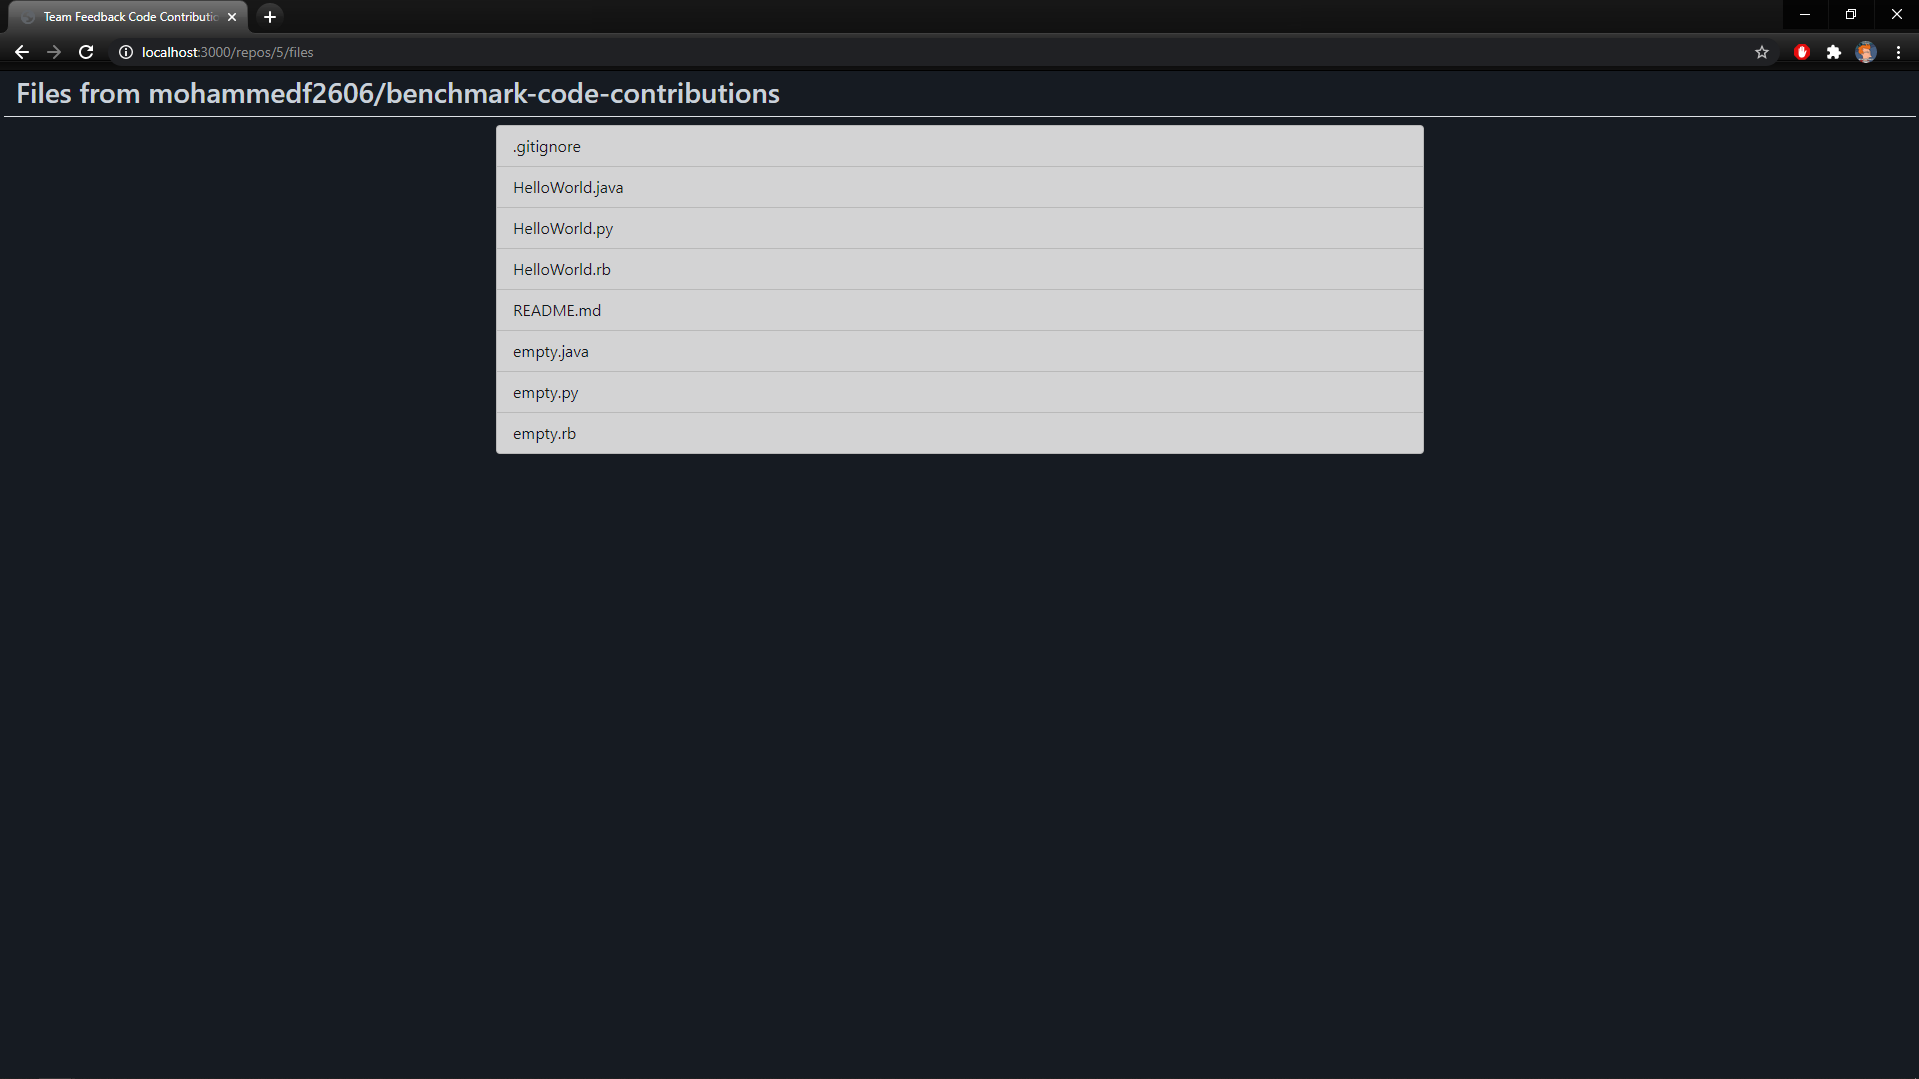
\includegraphics[scale=0.3]{Appendices/Screenshot_96.png}
    \caption{File list in selected repository}
    \label{fig:sc5}
\end{figure}
\begin{figure}
    \centering
    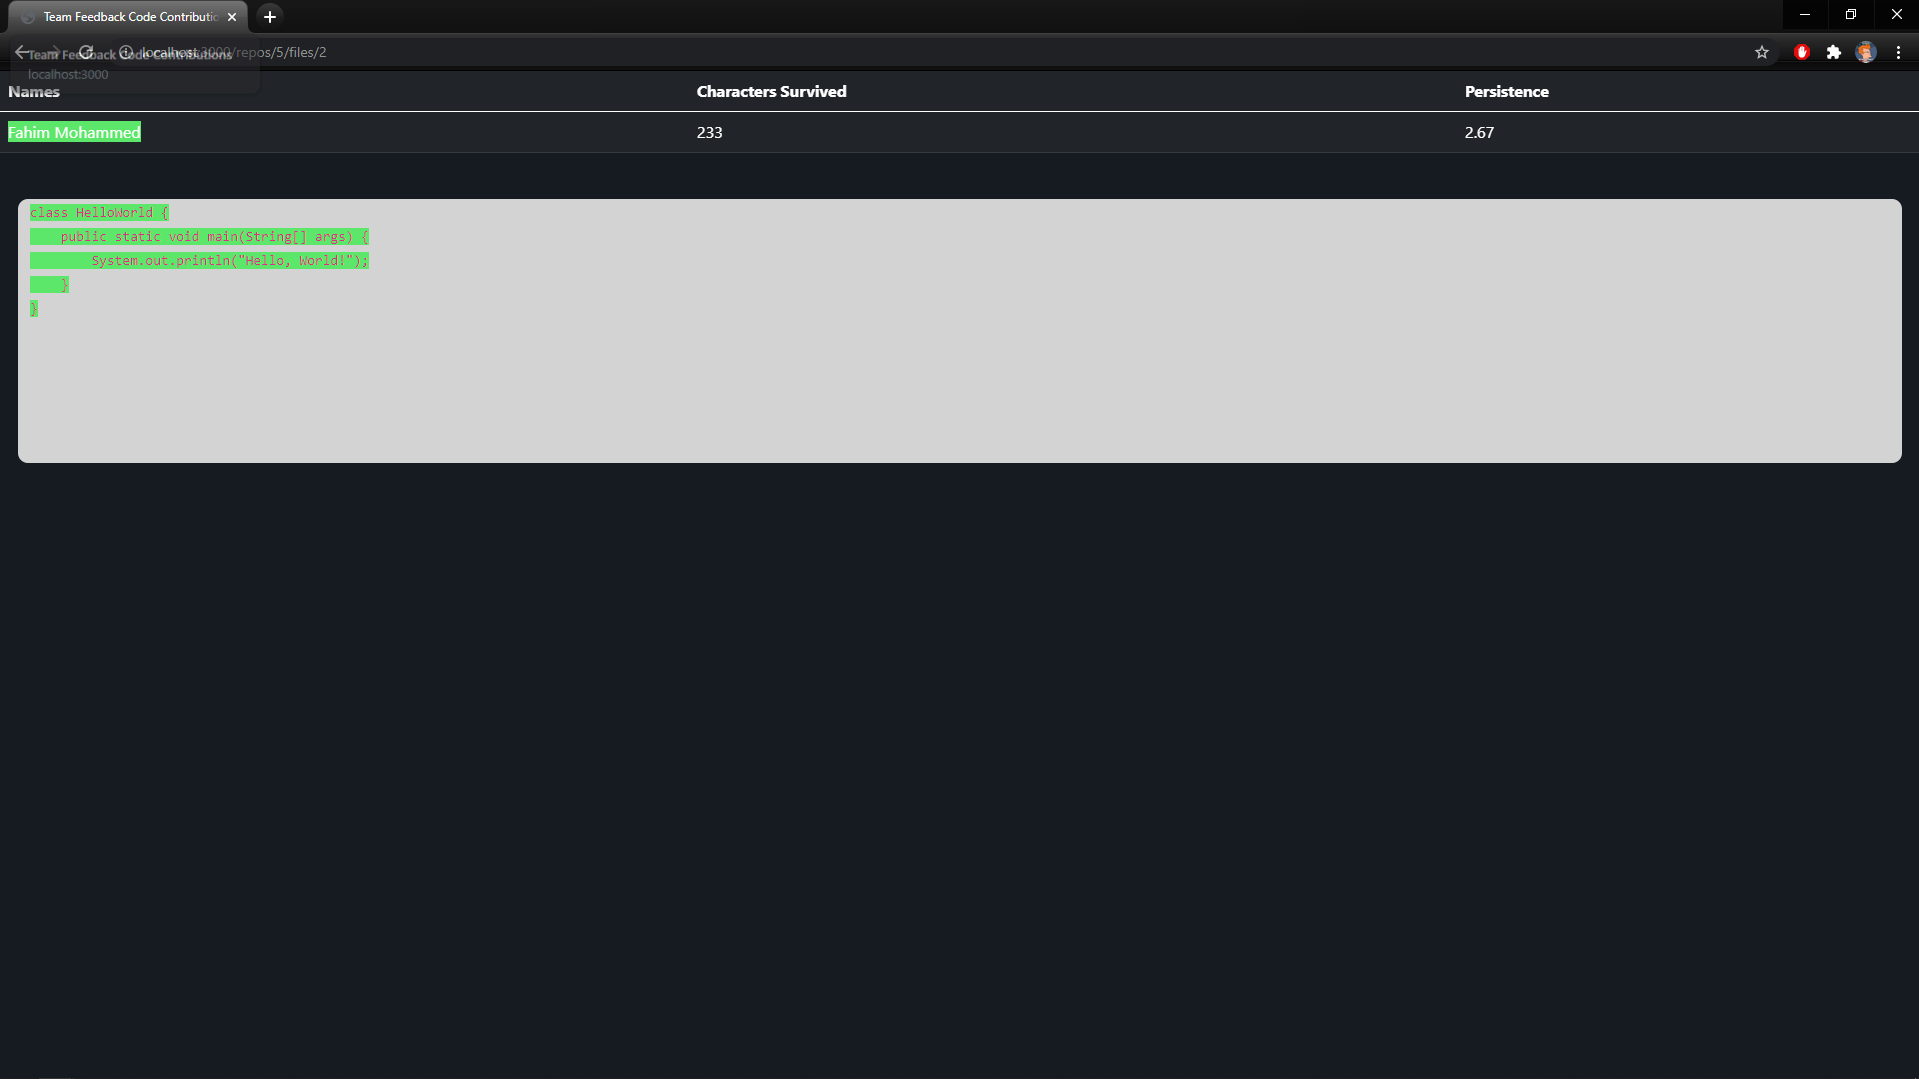
\includegraphics[scale=0.3]{Appendices/Screenshot_97.png}
    \caption{File-based visualisation in selected file}
    \label{fig:sc6}
\end{figure}
